\newpage

\section{\bfseries Arhitektura sistema}

U ovom poglavlju biće prikazana predložena arhitektura sistema.

\subsection{\bfseries Karakteristike sistema}

Arhitektura sistema je razmatrana tako da odgovara sledećim ciljevima koje sistem treba da ispuni:
\begin{itemize}
    \item Bezbednost
    \item Stabilnost
    \item Jednostavnost upotrebe
    \item Dostupnost
    \item Odziv
\end{itemize}
Bezbednost i stabilnost su postignuti troslojnom arhitekturom dok je jednostavnost upotrebe je postignuta pažljivom izradom korisničkog interfejsa. Izborom mobilne aplikacije omogućava se postizanje visokog stepena dostupnosti, dok je dobar odziv garantovan dokle god korisnik ima zadovoljavajuću internet konekciju.
Karakteristike arhitekture sistema za aplikaciju CarGo:
\begin{enumerate}
    \item Tip aplikacije: Mobilna aplikacija
    \item Strategije isporučivanja: Jedan serverski i više klijentskih računara
    \item Tehnologije: Android, Java, Geohash, Google S2 Geometry biblioteka
    \item Prateće komponente:
    \begin{enumerate}
        \item Logovanje na sistem: Podsistem za autentikaciju korisnika
        \item Praćenje vozila
        \item Lociranje korisnika
        \item Backup baze podataka: Podsistem koji automatski ili na zahtev pravi kopiju baze podataka
        \item Pomoć: Uputstvo za korišćenje veb aplikacije, kontakt forma, FAQ
    \end{enumerate}
\end{enumerate}

\newpage

\subsection{\bfseries Tip i slojevi arhitekture}

Za informacioni sistem je izabrana višeslojna klijent-server arhitektura koja se sastoji iz 3 sloja:
\begin{itemize}
    \item Prezentacioni sloj
    \item Logički sloj
    \begin{itemize}
        \item Klijentski kontroler
        \item Serverski kontroler
    \end{itemize}
    \item Sloj podataka
\end{itemize}

\subsubsection{\bfseries Prezentacioni sloj}

Predstavlja najviši sloj aplikacije i ima ulogu da korisniku
prikazuje i oslikava sadržaj koji dobija od nižih slojeva. Detaljniji prikaz je dat u sekciji Predlog izgleda korisničkog interfejsa. Ovaj sloj ima zadatak da korišćenje sistema učini efikasnijim i jednostavnijim i da korisnicima prikaže sve potrebne informacije koje dobije od nižih slojeva.
\newline
Sastoji se iz sledećih komponenti:
\begin{itemize}
    \item Registrovanje
    \item Prijavljivanje
    \item Naručivanje vožnje
    \item Ocenjivanje vozača
    \item Izmena ličnih podataka
\end{itemize}

\subsubsection{\bfseries Klijentski kontroler}

Glavni zadatak klijentskog kontrolera je da komunicira sa serverskim slojem sistema. Zadužen je da prosleđuje podatke prezentacionom sloju koji dalje korisnika obaveštava o ishodima njegovih akcija.
\newline
Sastoji se iz komponenti:
\begin{itemize}
    \item Validacija
    \item Dohvatanje podataka
    \item Autorizacija i autentifikacija
\end{itemize}

\subsubsection{\bfseries Serverski kontroler}

Serverski kontroler ima sličnu svrhu kao i klijentski kontroler, s tim što je obezbeđeno da klijenti nemaju pristup ovom delu aplikacije, prvenstveno zbog bezbednosti. Ovde se zbog toga vrše detaljnije autorizacije i validacije podataka kao i komunikacija sa bazom podataka. U ovom delu se takođe i izvršavaju neophodna izračunavanja nad podacima dobijenim iz baze.
\newline
Sastoji se iz komponenti:
\begin{itemize}
    \item Izačunavanje putanje vožnje
    \item Izračunavnje cene vožnje
    \item Naplaćivanje
    \item Autorizacija i autentifikacija
\end{itemize}
\subsubsection{\bfseries Sloj podataka}
Sadrži sve potrebne mehanizme za bezbedno pristupanje podacima u bazi podataka. Sloj podataka enkapsulira ove mehanizme i obezbeđuje lak pristup podacima. Zadatak mu je da dopusti pristup sloju iznad da koristi podatke na jednostavan način.

\begin{figure}[H]
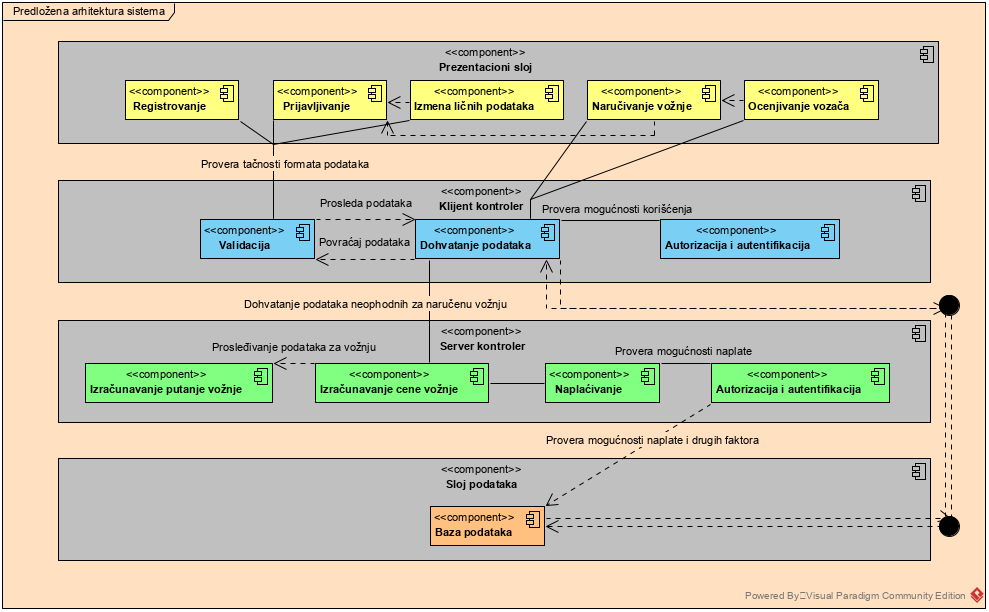
\includegraphics[scale = 0.70]{Slike/Arhitektura.png}
    \caption{Dijagram predložene arhitekture sistema}
\label{fig:Predložena arhitektura sistema}
\end{figure}

\newpage